We want to move even further removing any possible need for gridsearches or parameter optimization. The idea is that we will let the algorithm find the optimal parameters online. We want to leave the possibility to have different windows and different thresholds for each strategy. It is a complex combination of many simple sharpe threshold switches. This choice will drastically increase the computational burden, but it will grant much more robustness and flexibility to our switching method. This is because we will adapt our method to the characteristics of each strategy.\\
More in detail, we will leave to the algorithm the job of choosing a Sharpe window and a threshold each week for each strategy. So for a given date the algorithm will look at the past and backtest for each Sharpe window several thresholds and will choose the best one to apply for the following week.\\
Step by step the optimization is carried as follows for each week:
\begin{itemize}
	\item Generate a rolling window of 300 trading days.
	\item For each Sharpe-ratio window backtest the performance of an algorithm that simply trades the strategy only if the rolling Sharpe-Ratio is above the threshold.
	\item Each threshold is evaluated based on the performance (Sharpe-Ratio), and the best one is picked. If this gives a positive sharpe in the past, then we can proceed otherwise the strategy is just not switched.
	\item At last, we record the best threshold and apply it to the current Sharpe Ratio to see if the strategy can be put into production.
\end{itemize}

For the sake of completeness we started evaluating the performance of each threshold based on PnL (that's the most immediate and simple choice) but then we moved towards a Sharpe evaluation that is more strict on the choice of the parameter.\\
We decided to use several windows (60, 75, 90, 120, 150 days) and then combine the results to have more diversification. The good part is that there is no other optimization to be carried on, the method can either work or not. Luckily the results are quite encouraging.

\begin{table}
	\centering
	\begin{tabular}{c|c}
		\textbf{Statistic} & \textbf{Value} \\\hline
		Sharpe Ratio & 6.60 \\ 
		Sortino Ratio & 7.84 \\ 
		Omega Ratio & 3.29 \\ 
		Skewness & -0.5354 \\ 
		Kurtosis & 5.7234 \\ 
		Maximum Drawdown (\% duration/duration) & 3.6 \\ 
		Longest Drawdown (days) & 30.0 \\ 
		Winning Days & 71.88 \\ 
	\end{tabular}
	\caption{\label{tab:widgets} Statistics for the in-sample performance of the Threshold-Optimization method.}
\end{table}

The improvement in any aspect is remarkable and we have high hopes for the out-of-sample test as this method seems to be able to not overfit.
Here we can see the in-sample equity line (very steadily growing) and the number of selected strategies per each week.

\begin{center}
	\centering
	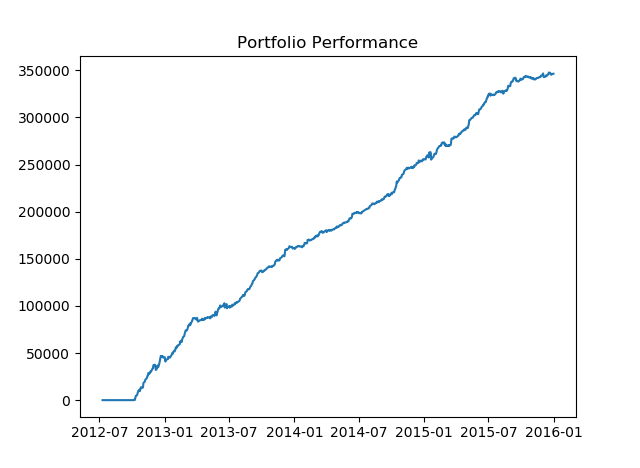
\includegraphics[width=0.6\textwidth]{GridSearches/Threshold_Backtest/In_sample_perf.png}
	\captionof{figure}{In-Sample performance for the Threshold-Optimization method.}
	\label{Average_Drawdown_in_sample}
\end{center}


\begin{center}
	\centering
	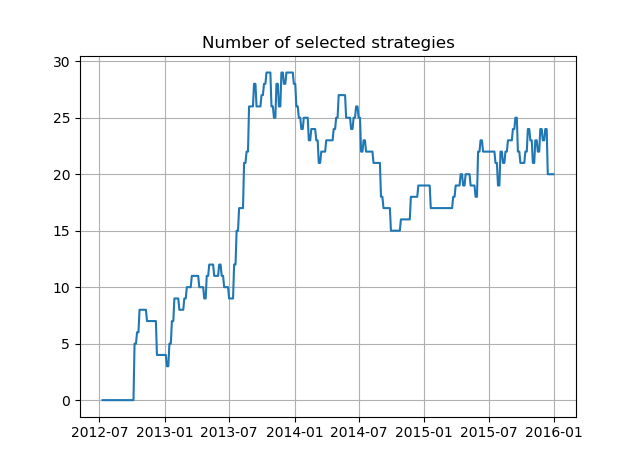
\includegraphics[width=0.6\textwidth]{GridSearches/Threshold_Backtest/num_strats_in_sample.png}
	\captionof{figure}{Number of strategies in production per week in the in-sample period.}
	\label{Average_Drawdown_in_sample}
\end{center}

We can see how this method is much more restrictive than the previous ones. We have not more than 25 strategies in production per week (while in the other methods we had always fixed the number to roughly 50, and in the regression based model we even had more than a hundred strategies).
